\documentclass[12pt]{article}

\usepackage{sbc-template}

\usepackage{graphicx}
\usepackage{url}
\usepackage{float}

\usepackage[utf8]{inputenc}
     
\sloppy

\title{Inception Network on TensorFlow}

\author{Claudio Roberto Scheer Junior\inst{1}, Samuel Camargo de Souza\inst{1}}

\address{Bachelor of Information Systems -- Três de Maio Faculty (SETREM)\\
   -- 98.910-000 -- Três de Maio -- RS -- Brazil
  \email{claudiojunior@setrem.com.br, samuel@samuelsouza.com}
}

\begin{document} 

\maketitle

\begin{abstract}
  This paper presents some examples of image classification using a pre-built model, provided by TensorFlow. The model was trained over the ImageNet 2012 Challenge data set, using an approach of CNN known as Inception Network. The data set has 10,000,000 labeled images depicting more than 10,000 object categories. Was possible to note that images with less unique features, has a low accuracy. While images with more unique features, has a high accuracy.
\end{abstract}

\section{General Information}

According to~\cite{tensorflow2015-whitepaper}, TensorFlow is a project released by Google in November 2015. The main objective of TensorFlow is to facilitate the use of machine learning due to the complexity of the algorithms.

Some classes of algorithms can have a better result in some situations. There may be variations according to the data or the results expected. So, programmers have to try different implementations, with different pamameters, to achive the best solution. TensorFlow can abstract it, offering a set of algorithms with different machine learning approaches, and some built in data set.

TensorFlow also provides a set of pre-trained models. In addition to abstracting the algorithms, it abstract the model training phase. It is helpful because the training phase requires a large processing power - generally GPUs, because of its particular characteristics on solving math problems.

The current paper uses a pre-trained model provided by TensorFlow. The model uses the Inception Network approuch to classify images, and was trained over the data set create for ImageNet 2012 Challenge. According to~\cite{imagenet}, the data set consist of 10,000,000 labeled images depicting more than 10,000 object categories.

The main objective of the current paper is to try different images, some taken by the author, over the pre-built model, and analysis how the model performs over this images.

\section{Resuts}

The images that are shown below was not treated. They are originals. Images that did not reached 75\% of accuracy when classified by the pre-trained model, was considered as having a not correct result.

\subsection{Antiperspirant Aerosol Image}

The Figure~\ref{fig:image1} shows an antiperspirant aerosol. When classifying it with the pre-trained model, the results are not correct.

\begin{figure}[H]
  \centering
  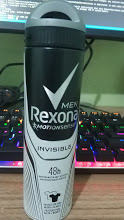
\includegraphics[width=.2\textwidth]{images/rexona.jpg}
  \caption{Antiperspirant aerosol}
  \label{fig:image1}
\end{figure}

The Table~\ref{tab:result1} shows the three top results:

% http://image-net.org/synset?wnid=n03476991
\begin{table}[H]
  \centering
  \caption{Top results of antiperspirant aerosol classification}
  \begin{tabular}{|c|c|}
    \hline
      Predicted Label & Accuracy \\
    \hline
    hair spray & 0.13998 \\
    water bottle & 0.06746 \\
    punching bag, punch bag, punching ball, punchball & 0.05384 \\
    \hline
  \end{tabular}
  \label{tab:result1}
\end{table}

\subsection{Motorcycle Image}

The Figure~\ref{fig:image2} shows a motorcycle. When classifying it with the pre-trained model, the top result is correct. There is a difference between a moped, as classified, and a motorcycle, as labeled. But, when looking to the data set used to train the model, is possible to note that the majority of the images used to train is a moped.

\begin{figure}[H]
  \centering
  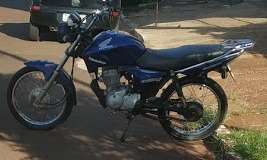
\includegraphics[width=.5\textwidth]{images/moto.jpg}
  \caption{Motorcycle}
  \label{fig:image2}
\end{figure}

The Table~\ref{tab:result2} shows the three top results:

\begin{table}[H]
  \centering
  \caption{Top results of motorcycle classification}
  \begin{tabular}{|c|c|}
    \hline
      Predicted Label & Accuracy \\
    \hline
    moped & 0.83319 \\
    motor scooter, scooter & 0.02867 \\
    disk brake, disc brake & 0.01527 \\
    \hline
  \end{tabular}
  \label{tab:result2}
\end{table}

\subsection{Bear Image}

The Figure~\ref{fig:image3} shows a bear. When classifying it with the pre-trained model, the top result is correct. The classification of the bear had a greater precision than the accuracy of the human being.

\begin{figure}[H]
  \centering
  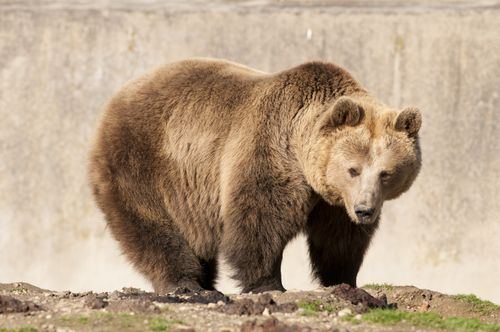
\includegraphics[width=.5\textwidth]{images/urso.jpg}
  \caption{Bear}
  \label{fig:image3}
\end{figure}

The Table~\ref{tab:result3} shows the three top results:

\begin{table}[H]
  \centering
  \caption{Top results of bear classification}
  \begin{tabular}{|c|c|}
    \hline
      Predicted Label & Accuracy \\
    \hline
    brown bear, bruin, Ursus arctos & 0.95103 \\
    ice bear, polar bear, Ursus Maritimus, Thalarctos maritimus & 0.00192 \\
    American black bear, black bear, Ursus americanus, Euarctos americanus & 0.00150 \\
    \hline
  \end{tabular}
  \label{tab:result3}
\end{table}

\section{Conclusion}

The examples shown above demonstrates the power of convolutional neural networks, more especifically, of Inception Network. When the classified image has singular features, like the bear and the motorcycle, the algorithm has high accuracy. But, when the classified image can be easily confused with another similar image, like the antiperspirant aerosol and the hair spray, the accuracy is low.

On the case of the antiperspirant aerosol, maybe the model might have a better accuracy if it was trained again with more images of antiperspirant aerosol. So, the model can learn some features that hair spray does not have.

\bibliographystyle{sbc}
\bibliography{sbc-template}

\end{document}
